
\documentclass[10pt,a4paper]{article}
\usepackage[utf8]{inputenc}
\usepackage[french]{babel}
\usepackage{amsmath}
\usepackage{graphicx}
\author{Jérôme Hue, Damien Carreau}
\title{Traitement du signal - Compte rendu}

\begin{document}
\maketitle
\section{La fonction Transformée de Fourrier Discrète}
La période d'échantillonage est : \( T_e = \dfrac{(b-a)}{N} = \dfrac{1}{327,68} \) \\
La fréquence d'échantillonage est : \( f_e = \dfrac{1}{T_e} = 327,68 \) \\
Intervalle de fréquence
L'intervalle entre deux échantillons en fréquence est de fe/N = 1/100.


\begin{figure}
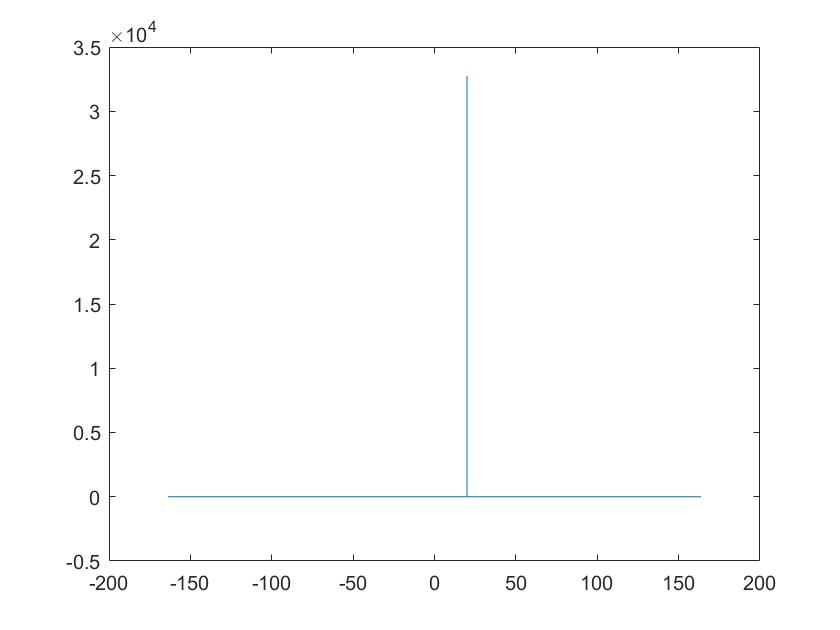
\includegraphics[scale=0.4]{tf_fct3.jpg}
\caption{Le spectre de la fonction 3}
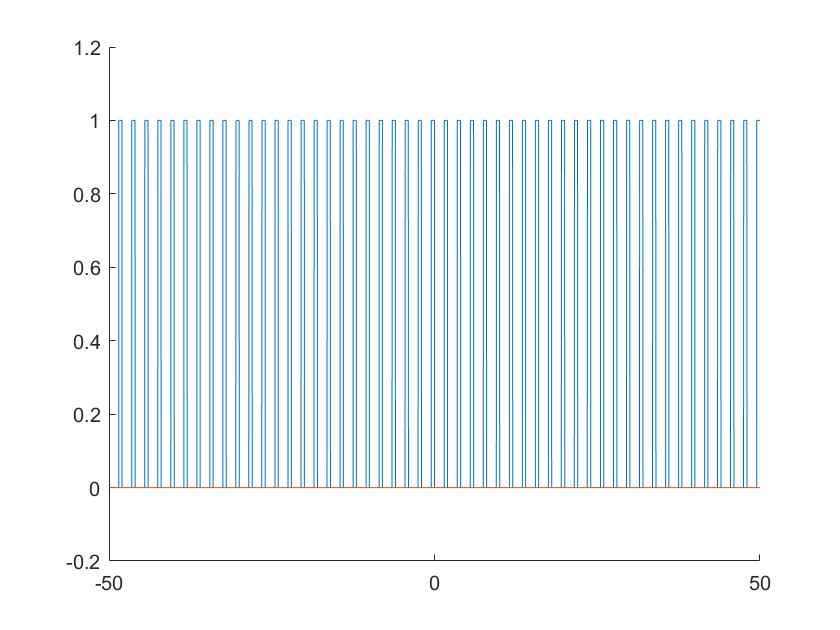
\includegraphics[scale=0.4]{fct6.jpg}
\caption{La fonction 6 après transformée de fourrier inverse}
\end{figure}



\section{Transmission par modulation d'amplitude}
\textit(Calcul théorique)

\textit{Extraire s1 ou s2 : }\\
Pour extraire s1 ou s2, il faut filtré la reprensentation fréquentielle de d, puis récupérer le signal temporel ainsi obtenu.

\textit{fréquence dépendante : }\\
Il faut faire attention à ne pas prendre des fréquences trop proches de celles de s1 ou s2.



\section{Echantillonnage et aliasing	}

\end{document}